\chapter*{Let's get started}

\ifnotes

    Learning outcomes:
    
    \begin{itemize}
        \item Describe project layout including feature files, stepdefs, programmer tests, application code
        \item Understand the role of Cucumber JUnit runners
        \item Explain the purpose of any other files that don't fit in the diagram
        \item Have a high level understanding of feature files, containing scenarios, containing steps
        \item Understand that the link between step and stepdef is based on textual matching
        \item Know that there are ways of running a subset of all the scenarios
    \end{itemize}
    
    We're expecting these answers in the diagram:
    \begin{itemize}
        \item Programmer Tests - Coordinate Test
        \item Feature - hear\textunderscore shout
        \item Step definitions - Shout Steps
        \item Your app - Shouty, Coordinate
    \end{itemize}
    
    Unexplained files:
    \begin{itemize}
        \JAVA{
            \item cucumber.xml - Spring integration
            \item RunCukes.java - JUnit runner
            \item Vanguard only - RunUnitCukesTest, RunAdhocCukesTest etc.
        }
        
        \item .....
    \end{itemize}
    
    Each step causes Cucumber to look for a matching stepdef to run. The match is text based. The matching is explained in more detail later on in the course.
    
    By default Cucumber will run all Scenarios in all Feature files it can find. There are multiple ways to run a subset of the Scenarios, the most common of which is tags. Most implementations also allow the target to be narrowed to specific Feature file(s), named Scenarios, or a combination of Feature file and line number.
    
   \section*{Vanguard specific}
   
   Vanguard TCoE have defined a number of tags that teams should use. These are needed by the predefined runners that are used in the CI pipelines and are necessary for the collection of metrics to see how well teams are confirming to 'best practice'
   
   \begin{itemize}
       \item @UnitTest - automation is at class/method level
       \item @IntegrationTest - automation requires multiple components to interact
       \item @EndToEndTest - automation requires full deploy of application
       \item @ManualTest - scenario will not been automated, so don't try to run
       \item @Ignore - scenario should not be run (broken, unreliable, unimplemented)
       \item @Adhoc - for use by developer interested only in running specific scenario(s). THIS SHOULD NEVER BE CHECKED INTO SOURCE CONTROL
       \item @Slow - (subjective) tag used to exclude time intensive tests
   \end{itemize}
   
   The first four tags above are mutually exclusive (only one should be applied to any scenario). They aren't business documentation, and so should not really be included in the feature file.
   
   Since we're talking tags, also explain that:
   \begin{itemize}
       \item tags are free text - you can make up any tag you want. It's meta data.
       \item tags flow down from Feature to Scenario (and to Examples tables)
       \item tagging the Feature with any of the Vanguard tags is almost always a bad idea.
   \end{itemize}

\fi 

\ifcontent 
    \CYBERDOJO
    {Navigate to Cyber-Dojo as instructed and enter the practice session that your instructor has prepared.}
    {Download the sample project and open it in \JAVA{your favourite editor or IDE}\CSHARP{Visual Studio (2013+)}\JAVASCRIPT{your favourite editor or IDE}\RUBY{your favourite editor or IDE}. You'll find a single \emph{feature} file in the \JAVA{\texttt{src/test/resources} directory}\CSHARP{\texttt{Shouty.Specs} project}\JAVASCRIPT{\texttt{features/} directory}\RUBY{\texttt{features/} directory}\ and you'll find programmer tests in one of the files in the \JAVA{\texttt{src/test/java} directory}\CSHARP{\texttt{Shouty.Tests} project}\JAVASCRIPT{\texttt{test/}}\RUBY{\texttt{spec/}}\ directory.}
    
    Take a look at the \JAVA{project}\JAVASCRIPT{project}\RUBY{project}\CSHARP{solution}\ and try to work out what each part is doing. Look at the following diagram and decide where each file in the project belongs. Write the \textbf{file names} onto this diagram:
    
    \begin{center}
    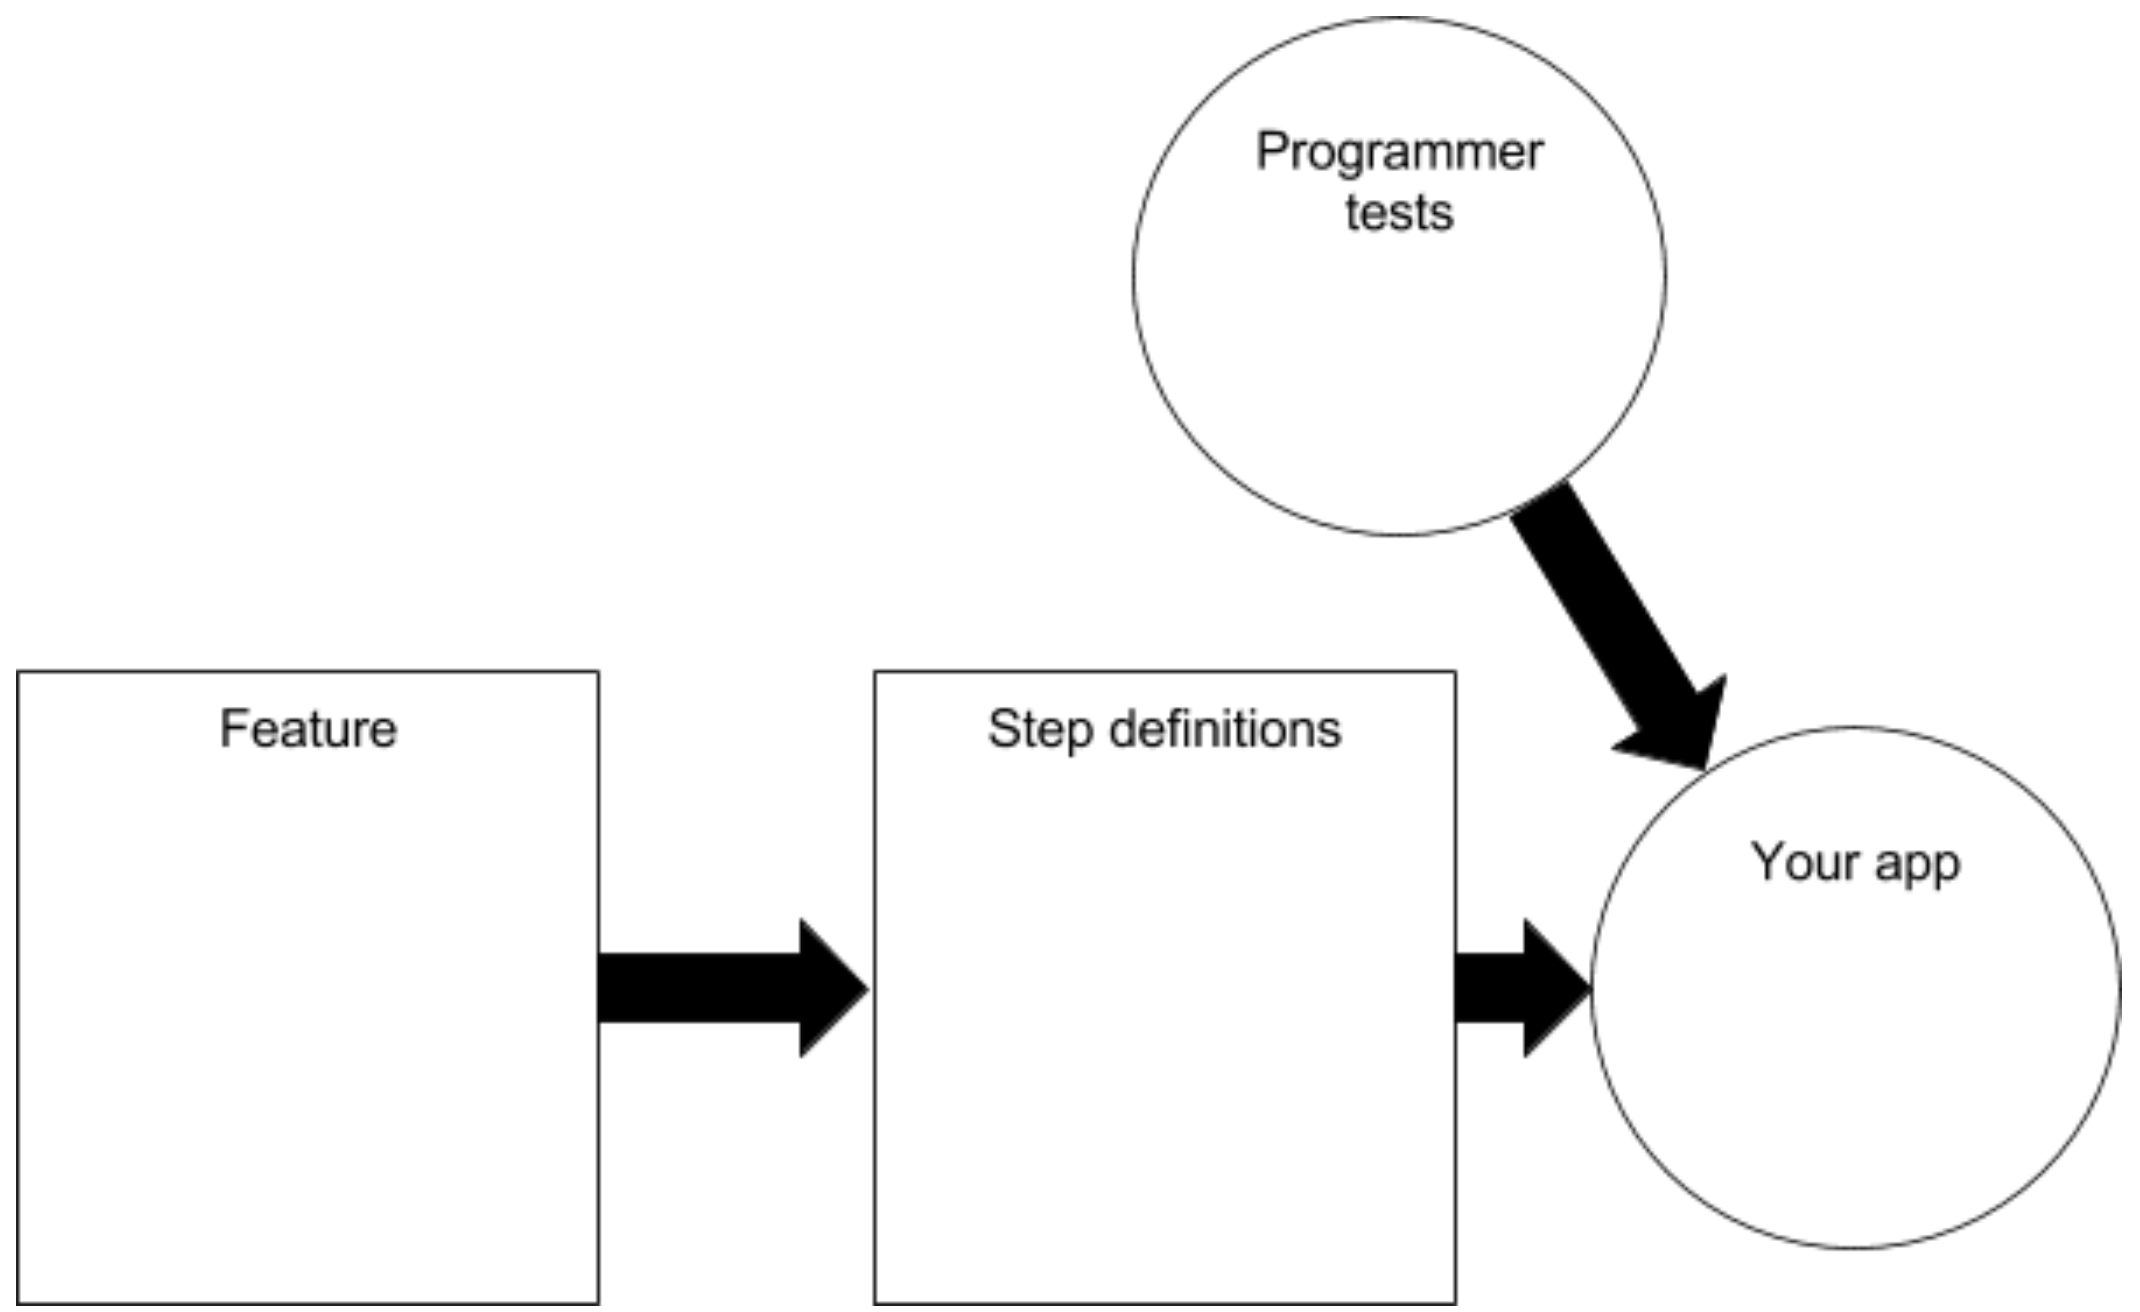
\includegraphics[width=.9\textwidth]{images/cucumber-anatomy}
    \end{center}
    
    Are there any files whose reason for existing is not clear? Which ones:
    
    \answerbox{1}
    
    The feature file contains scenarios made up of steps. Each step causes \CUKE{} to look for a {\workbookLanguage } \emph{step definition} to run. How does \CUKE{} decide which \emph{step definition} to run for each step?
    
    \answerbox{1}
    
    \JAVA{
        \QandAbox{And how does \CUKE{} decide which scenarios to run?}{1}
    }
    \JAVASCRIPT{
        \QandAbox{And how does \CUKE{} decide which scenarios to run?}{1}
    }
\fi